\section{Stack of Task}
Stack of Tasks(SOT) is a task based controller which is an efficient implementation of the GIK formalism in an heirarchical fashion inspired from Siciliano's work.  According to a classic task function based controller, the main objective of the task is to minimize the error between the desired pose of the robot and the current pose of the robot. These robot poses can be generalized to a term called as Features. Features refer to functional objective of a task in the world. Let us discuss the notion of a task and features with \textit{Visual Servo Control} as an example. \textit{Visual Servo Control} is a technique which uses vision data from the camera to control the motion of a robot. This technique allows to directly couple visual information and the robot motion in the control loop which makes it an attractive option to perform precise robust manipulation. The controller basically calculates joint velocity to reduce the error defined below \cite{Hutchinson2006}
\[\textit{e(t) = s(m(t),a) - s\textsuperscript{*}}\]
Where:
\begin{itemize}[label=]
    \item \textit{s(m(t),a)}: refers to the observed value of the features
    \item \textit{m(t)}:      refers to the instantaneous image measurements
    \item \textit{a}:         refers to the parameters that correspond to the knowledge of the system
    \item  \textit{s\textsuperscript{*}}:       refers to the desired value of the features
\end{itemize}
The standard approach is to develop a cartesian velocity controller for the robot which can control the motion of the camera mounted on the robot arm, based on the chosen features\cite{Hutchinson2006}. The velocity of the features or the errors with reference to robot frame can be represented by the below form
\[\dot{e} = L_{e}\mathbf{v}_{c}\] 
Where:
\begin{itemize}[label=]
    \item \textit{ $L_{e}$ }: refers to a feature Jacobian matrix that maps cartesian velocity of the camera to velocity of the features. The Jacobian matrix $L_{e} = L_{s}$ as the errors we calculate are with respect to the pre-defined features.
    \item \textit{ $\mathbf{v}_{c}$ }: refers to camera velocity = $({v}_{c},{\omega}_{c})$ 
\end{itemize}
 Considering the velocity of the camera to be the input to the controller, it is of the form
\[\mathbf{v}_{c}= -\lambda\widehat{L_{e}}e\]
Where:
\begin{itemize}[label=]
    \item \textit{ $\lambda$ }: is the gain of the velocity controller.
    \item \textit{ $\widehat{L_{e}}$ }: is the approximation of the pseudoinverse of the feature Jacobian matrix(interaction matrix).
    \item \textit{ $e$ }: is the error between the observed and desired value of the features.
\end{itemize}
This is a standard principle used in any task based velocity controller. SOT executes a hierarchy of tasks respecting the priorities 
of each task. Joint velocities are recursively computed with the below formulation\cite{Mansard2009}

\[\dot{q}_{i} = \dot{q}_{i-1} + (J_{i}P^{A}_{i-1}) + (\dot{e}_{i}-J_{i}\dot{q}_{i-1}), i=1..n\]

\[P^{A}_{i} = P^{A}_{i-1} - (J_{i}P^{A}_{i-1})^+ (J_{i}P^{A}_{i-1})                          \]
Where:
\begin{itemize}[label=]
    \item $P^{A}_{i}$ projects on the null-space of the augmented jacobian matrix of all the tasks
\end{itemize}

\section{Task Description}
Task function based controllers are quite common in humanoid robots domain and very seldom used in redundant mobile manipulators. This work is meant to bridge the educational gap by analyzing the state of art techniques in control of redundant robots and develop an SOT controller for KUKA youBot, which could be a major step in the solving problems in Mobile Manipulation.
 This R\&D will focus on designing and developing a visual servoing controller that can manipulate static and dynamic objects. This task is decomposed into simple and achievable tasks below
 \begin{itemize}
 \item Survey on the state of the art techniques of control of redundant robots and critically assess them.
 \item Constraint Analysis in Industrial scenarios
 \item Develop robot base collision constraints using laser sensor data
 \item Develop robot arm auto collision constraints and environment collision constraints using Flexible collision library
 \item Develop an 'SOT' controller for whole body control of KUKA youBot 
 \end{itemize}
% \subsection{Task Specification}
% \paragraph{Visual Control System}
% The system requires an appropriate number and type of cameras mounted over strategic positions to track the object or visually guide the robot in positioning the base. The main
% focus of out task is to achieve successful manipulation, which gives us a bit of idea to choose camera positions.In RoboCup@Work scenario, or any other new environment, it is
% always preferred to have a camera over the arm which is positioned in such a way to monitor the object with wide visibility. Also, there are various camera types which has a 
% potential impact on the type of features it can perceive. An appropriate definition of features with respect to ability of gripper to do successful grasping will help in deciding the right camera. In such systems, there is a possibility 
% that the camera can lose the target due to the motion of base around the object to afford arm reachability. In such cases, we need another camera to monitor the state of the 
% object which can guide the robot. 
% \paragraph{Implementation Details}
%  \begin{itemize}
% \item The implementation will start with an idea of detecting two dimensional line features which can generalize all the proposed graspable objects. A primitive level visual control which can handle only four specific joints of the base and arm is developed. In control terms, a feature Jacobian of dimension four will be built to 
% control the velocity of limited joints. This implementation is done to find out issues in features and upcoming control problems.
% \begin{figure}[here]
%  \vspace{2 mm}
%   \centerline {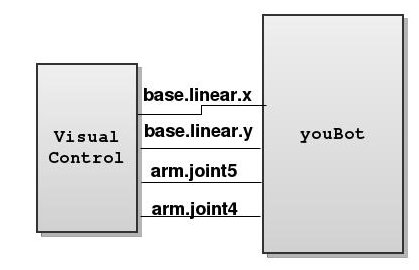
\includegraphics[scale=0.44]{images/vs_primitive}}
%   \caption{Primitive Visual Control}
%  \vspace{2 mm}
% \label{fig:primviscont}
% \end{figure}
% \newline
% The figure \ref{fig:primviscont} shows an overview of the controller. Pre-grasp arm joint positions are chosen for other joints to ensure the object in the visual field 
% of the camera.
% 
% \item The development will target on mapping feature error to all the joints of the robot to have a whole body control. A rough overview of the system is below.
% 
% \section{Evaluation Stategy}
% Evaluation of the developed algorithm is to be done on the proposed objects which affords to grasping ability of the KUKA youbot gripper and has significant line features. The 
% joint velocity components, evolution of errors, the number of iterations and other necessary parameters will be monitored. Stability analysis of the
% control algorithm is performed to evaluate the performance of the algorithm.
% \paragraph{Stability Analysis of Closed Loop Control}
% Lyapunov analysis will be used to determine the stability of the control algorithm\cite{Hutchinson2006}. The Lyapunov function $L =  1/2\parallel  e  \big(t\big) \parallel ^{2}$
% will be used to analyse the global and local assymptotic stability of the system by testing on various task constraints listed below.
% \begin{itemize}
% \item Initial camera positions by varying along one degree of freedom or multiple degree of freedom as done in \cite{jagersand1997experimental}. Various camera positions
% enable to evaluate the algorithms under local minima.
% \item Initial robot base positions based on how close it is with respect to the platforms and other obstacles. 
% \end{itemize}
% The above list will get updated in the course of the project to measure the performance effectively.
% 







